\documentclass[xcolor=dvipsnames,12pt]{beamer}
\usecolortheme[named=RoyalPurple]{structure}
\useoutertheme{infolines}
\usetheme{CambridgeUS}
%\usetheme[height=14mm]{Rochester}
%\hypersetup{colorlinks=true,linkcolor=yellow}
\setbeamertemplate{items}[ball]
\setbeamertemplate{blocks}[rounded][shadow=true]
\setbeamertemplate{navigation symbols}{}
\usepackage{color}
%\usefonttheme{structuresmallcapsserif}
%\usefonttheme{professionalfonts}
%\useoutertheme{default}
%\useoutertheme{infolines}


%\documentclass{beamer}
%\usecolortheme{structure}
\usepackage{graphicx}
%\usetheme{PaloAlto}
%\setbeamertemplate{items}[ball]
%\setbeamertemplate{blocks}[rounded][shadow=true]
%\useoutertheme{umbcfootline}
\newtheorem{assume}{\rlap{A}\hskip .1in}
%\newtheorem{result}{Result}[chapter]
\newcommand{\Var}  {\mbox{Var}}
\newcommand{\V} {\mbox{V}}
\newcommand{\E}  {\mbox{E}}
\newcommand{\PR}  {\mbox{P}}
\newcommand{\diag} {\operatorname*{diag}}
\newcommand{\tr} {\mbox{tr}}
\newcommand{\bmw}[1]{{\mbox{$#1$}}}
\newcommand{\MSE}{\mbox{MSE}}
\newcommand{\MSPE}{\mbox{MSPE}}


\def\bmh{{\hat \mathbf m}}
\def\bm{{\mathbf m}}
\def\bn{{\mathbf n}}
\def\mh{{\hat m}}
\def\bOmega{{\mathbf \Omega}}
\def\be{{\mathbf e}}
\def\bs{{\mathbf s}}
\def\by{{\mathbf y}}
\def\b1{{\mathbf 1}}
\def\bx{{\mathbf x}}
\def\bw{{\mathbf w}}
\def\bzero{{\mathbf 0}}

\def\bP{{\mathbf P}}
\def\bI{{\mathbf I}}
\def\bM{{\mathbf M}}
\def\bH{{\mathbf H}}
\def\bN{{\mathbf N}}
\def\bW{{\mathbf W}}
\def\bX{{\mathbf X}}
\def\bZ{{\mathbf Z}}
\def\bT{{\mathbf T}}
\def\bV{{\mathbf V}}
\def\bC{{\mathbf C}}
\def\bG{{\mathbf G}}
\def\bY{{\mathbf Y}}
\def\bD{{\mathbf D}}
\def\bS{{\mathbf S}}
\def\bR{{\mathbf R}}

\def\bbeta{\mbox{\boldmath $\beta$}}
\def\bepsilon{\mbox{\boldmath $\varepsilon$}}

% items enclosed in square brackets are optional; explanation below
\title[]{Part 4}
%\subtitle[ttt]{}
\author[Stat 801]{Inferences about {\boldmath$\mu_1$ - $\mu_2$}\\
Confidence Intervals for {\boldmath$\mu_1$ - $\mu_2$}\\
Welch's t test\\
Inferences about {\boldmath$\mu_1$ - $\mu_2$} for Paired Data}
\date{}

\begin{document}

\begin{frame}[plain]
  \titlepage
\end{frame}




\begin{frame}
\frametitle{INFERENCES ABOUT {\boldmath$\mu_1$ - $\mu_2$}}
\begin{itemize}
\item In many situations one wishes to  \textcolor{magenta}{\textit{compare}} the means
of two different populations.  
\item Let $\mu_1$ and $\mu_2$ denote means two populations. 
\item Most often, the comparison of interest is the difference
$\mu_1 - \mu_2$.
\item We will make the comparison based on a random sample
from each population.  Suppose samples of sizes $n_1$ and $n_2$ are
drawn.
\end{itemize}
\end{frame}


\begin{frame}
\begin{itemize}
\item  Let $\bar{Y}_1$ and $\bar{Y}_2$ denote sample mean random
variables and $S_1$ and $S_2$ be the sample standard deviation 
random variables computed from each sample.
\item  Also assume that the samples are drawn  \textcolor{magenta}{\textit{independently}}
from each population, and that the populations have the same
variance $\sigma^2$.
\item  For large sample sizes, the random variables $\bar{Y}_1$ and $\bar{Y}_2$ are
\textcolor{magenta}{\textit{approximately normal}}.
\item Thus the random variable $\bar{Y}_1 - \bar{Y}_2$ is
also approximately normal.
\end{itemize}
\end{frame}


\begin{frame}
\begin{itemize}
\item The mean of the random variable $\bar{Y}_1 - \bar{Y}_2$  is $\mu_1 - \mu_2$ 
and standard deviation is
$$
  \sigma_{\bar{Y}_1 - \bar{Y}_2} =
  \sqrt{\frac{\sigma_1^2}{n_1} + \frac{\sigma_2^2}{n_2}} 
$$
where $\sigma_1^2$ and $\sigma_2^2$ are the variances of each 
of each population. 
\item However,  under the assumption  that
$\sigma_1^2 = \sigma_2^2 \equiv \sigma^2$, the standard deviation becomes
$$
  \sigma_{\bar{Y}_1 - \bar{Y}_2} =
  \sqrt{\frac{\sigma^2}{n_1} + \frac{\sigma^2}{n_2}} =\sigma\sqrt{\left(\frac{1}{n_1}+\frac{1}{n_2}\right)}
$$
\end{itemize}
\end{frame}


\begin{frame}
\begin{itemize}
\item An estimator of $ \sigma_{\bar{Y}_1 - \bar{Y}_2}$ is
$$
  S_{\bar{Y}_1 - \bar{Y}_2} = S_p \sqrt{\left(\frac{1}{n_1} + \frac{1}{n_2}\right)}
$$
\item $S_p^2$ is the  \textcolor{magenta}{\textit{pooled estimator}} of the common variance
$\sigma^2$ of the two populations.
\item This is obtained under the assumption  that
$\sigma_1^2 = \sigma_2^2 \equiv \sigma^2$, the common variance . 
\item Later we will talk about what to do if we can't reasonably make
this assumption in a given situation.
\end{itemize}
\end{frame}



\begin{frame}
\begin{itemize}
\item Consider the random
variable defined as:
$$
  T_{n_1 + n_2 - 2} = \frac{(\bar{Y}_1 - \bar{Y}_2) - (\mu_1 -
\mu_2)}{S_{\bar{Y}_1 - \bar{Y}_2}}
$$
\item When sampling is from Normal distributions, the distribution of the
above statistic is distributed exactly as Student's $t$ with 
$df=n_1 + n_2 - 2$. 
\item For large samples we may use the CLT and say that $ T_{n_1 + n_2 -
2}$ will be approximately distributed as Student's $t$ with 
$df=n_1 + n_2 - 2$
\item For small samples, however, we must verify if the samples  were 
actually drawn from Normal distributions, using
tools such as boxplots and normal probability plots
\end{itemize}
\end{frame}


\begin{frame}
\begin{itemize}
\item We shall do that before calculating confidence intervals 
for $\mu_1 - \mu_2$, and for testing hypotheses using the $t$ 
distribution. 
\item The \textcolor{magenta}{\textit{pooled estimator}} of the common variance $\sigma^2$,
$S_p^2$, is obtained  using the weighted average
$$
  S_p^2 = \frac{(n_1-1)S_1^2 + (n_2-1)S_2^2}{n_1+n_2 - 2}
$$
\end{itemize}
\end{frame}


\begin{frame}
\begin{itemize}
\item Here  $S_1^2$ and $S_2^2$ are sample variance random variables.
  $S_1^2  = \frac{1}{n_1-1} \sum_{j=1}^{n_1} (Y_{1j} - \bar{Y}_1)^2$\quad \quad
 $ S_2^2 =  \frac{1}{n_2-1} \sum_{j=1}^{n_1} (Y_{2j} - \bar{Y}_2)^2$ \\[-.3in]
\item Thus a  \textcolor{magenta}{\textit{100(1-$\alpha$)\% Confidence Interval for $\mu_1 - \mu_2$}}
is
 $ \bar{y}_1 - \bar{y}_2 \pm t_{\alpha/2,df}\cdot \, s_p $
  $\sqrt{\frac{1}{n_1} + \frac{1}{n_2}} $
\item Here $df= n_1 + n_2 - 2$ and
$$
  s_p = \sqrt{\frac{(n_1-1)s_1^2+(n_2-1)s_2^2}{n_1 + n_2 - 2}}
$$
\end{itemize}
\end{frame}


\begin{frame}
\frametitle{{Example}}
 Company officials, concernerned about potency of a product retained after storage, drew a random sample of $n_1=10$ bottles from the production line and tested for potency. Another random sample of $n_2=10$ bottles was drawn and stored in a regulated environment for 1 year and then tested. The data obtained are:\\[.1in]
{\small 
\begin{center}
\begin{tabular}{rrrrr} \hline
\multicolumn{2}{c}{\textbf{Fresh}} & & 
\multicolumn{2}{c}{\textbf{Stored}} \\ \hline
10.2 & 10.6 & & 9.8 & 9.7 \\
10.5 & 10.7 & & 9.6 & 9.5 \\
10.3 & 10.2 & & 10.1 & 9.6 \\
10.8 & 10.0 & & 10.2 & 9.8 \\
9.8 & 10.6 & & 10.1 & 9.9 \\ \hline
\end{tabular}
\end{center}}
\end{frame}


\begin{frame}
\frametitle{Solution}
\hspace*{1in}$n_1 =10 \hspace*{1in} n_2 = 10 $\\[.15in]
\hspace*{.15in}$\ \bar{y}_1 =103.7/10= 10.37 \quad \quad   \bar{y}_2 =98.3/10= 9.83$ \\[.15in]
\hspace*{1in}$s_1^2 = [1076.31-\frac{(103.7)^2}{10}]/9=0.105$ \\[.15in]
\hspace*{1in}$s_2^2 =[966.81-\frac{(98.3)^2}{10}]/9= .058$ 
\begin{eqnarray*}
 s_p & = & \sqrt{\frac{(n_1-1)s_1^2+(n_2-1)s_2^2}{n_1 + n_2 - 2}}=\sqrt{\frac{9}{18} (s_1^2 + s_2^2)}\\[.15in]
& = &  \sqrt{\frac{.105+.058}{2}} = 0.285
\end{eqnarray*}
\end{frame}


\begin{frame}
\frametitle{Solution - cont.}
The t-percentile based on $df= n_1+n_2-2= 10+ 10 -2= 18$ and $\alpha=.025$ is $ t_{.025,18}=2.101$\\[.05in]
 Thus a 95\% confidence interval for the difference in the mean potencies $\mu_1-\mu_2$ is:\\[.05in]
\hspace*{1in} $(10.37-9.83) \pm2.102 (.285)\sqrt{\frac{1}{10}+\frac{1}{10}} $\\[.05in] 
\hspace*{1.7in}$.54\pm .268$ \quad or \quad $(.272,\,.808)$\\[.05in] 
 Thus, the difference in mean potencies for bottles from the production line and those stored for one year, $\mu_1-\mu_2$, is estimated  to be between .272 and .808 with \textcolor{magenta}{\textit{95\% confidence}}.\\[.05in]
 It is important understand what we mean by the above statement.
\end{frame}



\begin{frame}
\frametitle{Example}
\begin{center}
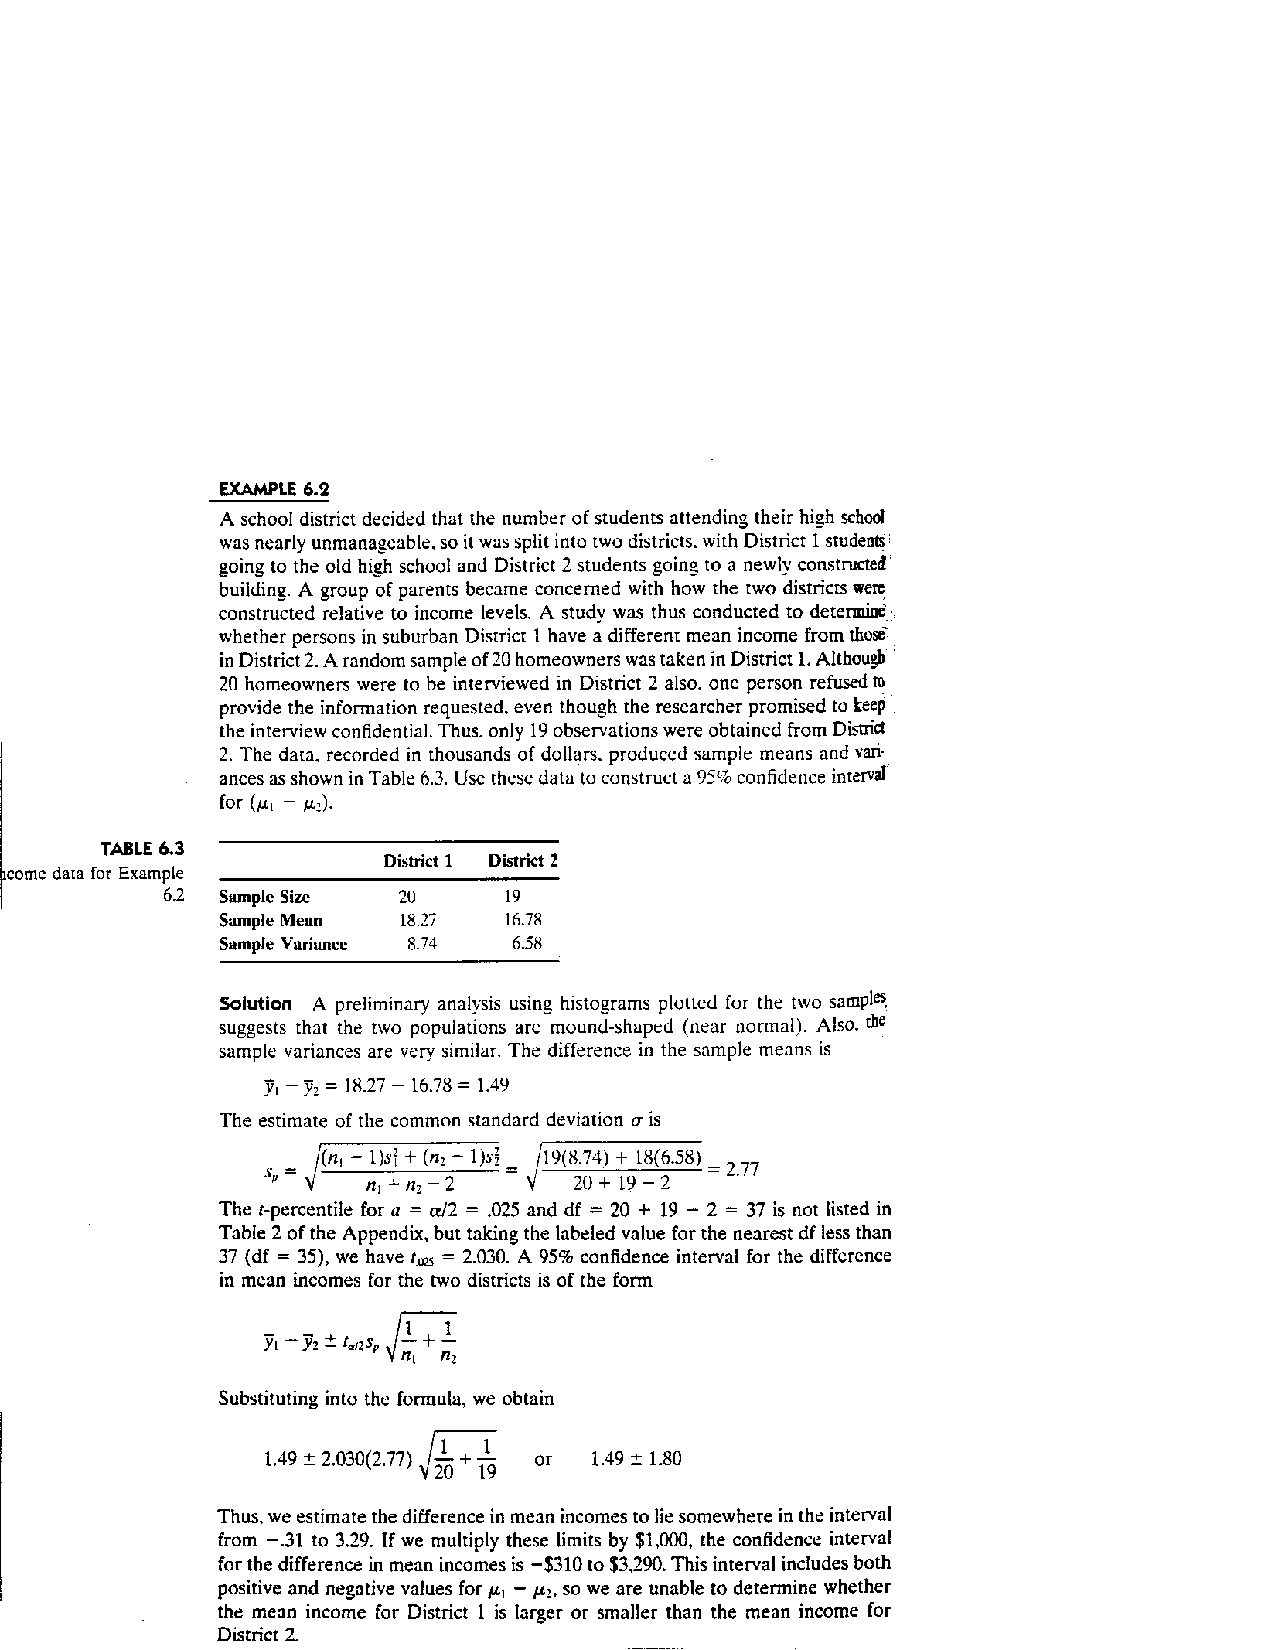
\includegraphics[trim={5cm 0cm 0cm 8cm},clip,scale=0.38]{ex6_2.pdf}\\[.1in]
\end{center}
\end{frame}


\begin{frame}
\frametitle{Tests of Hypotheses about $\mu_1-\mu_2$}
The types of hypothesis that may be tested are similar to those on the mean of a single population. 
These are:
\begin{tabbing}
xxxxx \= xxxxxxxxxxxxxxxxxxxxx \=  \kill
\>1. $H_0:$  $\mu_1 - \mu_2 \leq  D_0$ \> $H_a:$  $\mu_1 - \mu_2 > D_0$ \\
\>2. $H_0:$  $\mu_1 - \mu_2 \geq  D_0$ \> $H_a:$  $\mu_1 - \mu_2 < D_0$ \\
\>3. $H_0:$  $\mu_1 - \mu_2 =  D_0$   \> $H_a:$   $\mu_1 - \mu_2 \neq D_0$ 
\end{tabbing}
(where $D_0$ is a specified number, often zero.)\\[.1in]
The test statistic for testing each of the above hypotheses is
$$
T = \frac{\bar{Y}_1 - \bar{Y}_2 - D_0}{S_p\sqrt{\frac{1}{n_1}+\frac{1}{n_2}}} 
$$
\end{frame}


\begin{frame}
The \textcolor{magenta}{\textit{two-sample t-statistic}} is calculated using the sample statistics: $\bar{y}_1, \bar{y}_2$ and $s_p$:\\
\vspace{5mm}
\hspace{35mm}
 $ t =\frac{\bar{y}_1 - \bar{y}_2 - D_0}{s_p\sqrt{\frac{1}{n_1}+\frac{1}{n_2}}}$\\
\vspace{5mm}
The rejection regions for each test, respectively, are:
\begin{enumerate}
\item Reject $H_0$  if  $t > t_{\alpha,\,df}$ 
\item Reject $H_0$  if  $t < -t_{\alpha,\,df}$
\item Reject $H_0$  if  $|t| > t_{\alpha/2,\,df}$
\end{enumerate}
Note that the degrees of freedom is $df=n_1+n_2-2$
\end{frame}



\begin{frame}
Handout - Example 6.3
\end{frame}

%\vspace*{-1in}
%\epsfig{figure=graphs/ex6_3.eps,width=4.5in,height=5in,angle=0,silent=}
%\vspace*{.5in}
%

%\h   \textcolor{magenta}{\small{Refer to Example 6.3: JMP Analysis also}}



\begin{frame}
\frametitle{Exercise}
 Two different emission-control devices were being
tested to determine the average amount of nitric oxide being emitted
by an automobile over a 1-hour period of time.  Twenty cars of the
same model and year were selected for the study.  Ten cars were
randomly selected and equipped with a Type 1 emission-control device,
and the remaining cars were equipped with Type II devices. Each of
the 20 cars was then monitored for a 1-hour period to determine
the amount of nitric oxide emitted.\\[.1in]
Use the following data to test the research hypothesis that the mean
level of emission for Type 1 devices ($\mu_1$) is greater than the
mean emission level for Type II devices ($\mu_2$).  Use $\alpha=.01$.\\[.1in]
\end{frame}

\begin{frame}
\frametitle{Exercise - cont.}
\begin{center}
\begin{tabular}{rrrrr} \hline
\multicolumn{2}{c}{\textbf{Type 1 Device}} & & 
\multicolumn{2}{c}{\textbf{Type II Device}} \\ \hline
1.35 & 1.28 & & 1.01 & 0.96 \\
1.16 & 1.21 & & 0.98 & 0.99 \\
1.23 & 1.25 & & 0.95 & 0.98 \\
1.20 & 1.17 & & 1.02 & 1.01 \\
1.32 & 1.19 & & 1.05 & 1.02 \\ \hline
\end{tabular}
\end{center}
\end{frame}

\begin{frame}
\frametitle{Exercise - cont.}
\hspace*{2in}$n_1 = n_2 = 10 $\\[.1in]
\hspace*{1.4in}$\ \bar{y}_1 = 1.236 \quad \quad   \bar{y}_2 = 0.997$ \\[.1in]
\hspace*{1.5in}$s_1^2 = 0.004096 \quad s_2^2 = 0.0009$ \\[.1in]
\hspace*{1.2in}$s_p^2 = \frac{9}{18} (s_1^2 + s_2^2) = 0.0025 \quad \quad s_p$ = 0.05 \\[.1in]
\hspace*{.8in}$H_0: \mu_1 - \mu_2 \leq 0$\ \ vs. $H_a: \mu_1 - \mu_2 > 0 $\\[.15in]
\hspace*{1.5in}$t_c = \frac{1.236-0.997}{0.05\sqrt{0.2}} = 10.71$ \\[.15in]
\hspace*{1.2in}$t_{0.01,18} = 2.552$ implying R.R. is $t>2.552$\\[.1in]
Therefore reject $H_0$ at $\alpha=.01$ as  $t_c$ is in the R.R.\\[.1in]
Thus it appears that the mean level of emission for the Type I
device is greater than for Type II.
\end{frame}



\begin{frame}
\frametitle{The above confidence interval and test formulae are based on several assumptions}
\begin{enumerate}
\item The two samples are drawn independently from the two
      populations.
\item The two populations are such that $\bar{Y}_1$ and
      $\bar{Y}_2$ are approximately normal.  (We make use of
      the CLT if the size of samples $n_1$ and $n_2$ are 
      sufficiently large.)
\item The two populations have the same variance $\sigma^2$
      (in order to see if this assumption may not hold one
      looks at $s_1^2$ and $s_2^2$.)
\end{enumerate}
\end{frame}



\begin{frame}
\frametitle{About Assumptions}
Assumption 3. is the unusual. When $n_1 = n_2 = n$, unless studies indicate that
$\sigma_1^2$ and $\sigma_2^2$ can differ by as much as a factor
of 3, it won't make a difference in the inference
about $\mu_1 - \mu_2$ based on the use of given formulae
for C.I.'s and tests.\\[.1in] When we find ourselves in a situation where Assumption 3.
seems to be seriously violated, we can use an
\textcolor{magenta}{\textit{an approximate $t$ test}} described below.\\[.1in]
Assumption 1. requires that the samples from the two populations
are obtained in such a way that the elements of the two samples are
\textcolor{magenta}{\textit{statistically independent}}. 
\end{frame}



\begin{frame}
\frametitle{Welch's $t$ test}
The hypotheses to be tested are as usual:
\begin{tabbing}
xxxxx \= xxxxxxxxxxxxxxxxxxxxx \=  \kill
\>1. $H_0:$  $\mu_1 - \mu_2 \leq  D_0$ \> $H_a:$  $\mu_1 - \mu_2 > D_0$ \\
\>2. $H_0:$  $\mu_1 - \mu_2 \geq  D_0$ \> $H_a:$  $\mu_1 - \mu_2 < D_0$ \\
\>3. $H_0:$  $\mu_1 - \mu_2 =  D_0$   \> $H_a:$   $\mu_1 - \mu_2 \neq D_0$
\end{tabbing}
 The test statistic is :
$$
  t' = \frac{(\bar{y}_1 - \bar{y}_2) - D_0}
  {\sqrt{\frac{s_1^2}{n_1} + \frac{s_2^2}{n_2}}} 
$$
Note that the two sample variances are NOT pooled to obtain a pooled sample variance estimate.
\end{frame}


\begin{frame}
\frametitle{Welch's $t$ test - cont.}
The percentile points of the $t'$-statistic are approximated by using the t-table with an \textcolor{magenta}{\textit{adjusted degrees of freedom}} given by:
$$
df = \frac{(n_1-1)(n_2-1)}{(n_2-1)c^2 + (1-c)^2(n_1-1)}
$$
\begin{flushright}(round down to an integer)\end{flushright}
 where
$$
  c = \frac{s_1^2/n_1}{\frac{s_1^2}{n_1} + \frac{s_2^2}{n_2}}
$$
\end{frame}




\begin{frame}
\frametitle{Welch's $t$ test - cont.}
For specified $\alpha$ the rejection regions for the three hypotheses, respectively, are given by:
\begin{tabbing}
xxxxx \= xxxxxxxxxxxxxxxxxxxxx \=  \kill
\>1.  \ Reject $H_0$ \ if \ $t' > t_{\alpha,\,df}$ \\
\>2. \ Reject $H_0$ \ if \ $t' < -t_{\alpha,\,df}$\\
\>3. \ Reject $H_0$ \ if \ $|t'| > t_{\alpha/2,\,df}$
\end{tabbing}
 An approximate $100(1-\alpha)\%$ confidence interval for
 $\mu_1 - \mu_2$  is:
 $$(\bar{y}_1 - \bar{y}_2) \pm t_{\alpha/2,\,df}\cdot \sqrt{\frac{s_1^2}{n_1} +
\frac{s_2^2}{n_2}}$$
 where $t_{\alpha/2}$ is the $t$ quantile found from the t-table for $df$
computed using the above formula.
\end{frame}


\begin{frame}
Handout - Oil spill data
\end{frame}




\begin{frame}
\frametitle{Inferences about $\mbox{\boldmath$\mu_1 - \mu_2$}$ for
Independent Samples}
\begin{itemize}
\item Consider \textcolor{magenta}{\textit{independent samples}} from two populations having means and variances ($\mu_1, \sigma_1^2$) and ($\mu_2, \sigma_2^2$), respectively.
\item  The mean and variance of the sampling random variable 
$\bar{Y}_1 - \bar{Y}_2$ are:
$$
  E(\bar{Y}_1 - \bar{Y}_2) = \mu_1 - \mu_2 \quad
  V(\bar{Y}_1 - \bar{Y}_2) = \frac{\sigma_1^2}{n_1} + 
  \frac{\sigma_2^2}{n_2}
$$
\item  Point estimates of these we know are:
$$
  \bar{y}_1 - \bar{y}_2 \quad \rm{and} \quad \quad
  \frac{s_1^2}{n_1} + \frac{s_2^2}{n_2} \ .
$$
\end{itemize}
\end{frame}


\begin{frame}
\frametitle{Inferences about $\mbox{\boldmath$\mu_1 - \mu_2$}$ for
Independent Samples - cont.}
\begin{itemize}
\item  If the two populations have the same variances, so that $\sigma_1^2 = \sigma_2^2 = \sigma^2$ then
$$
  V(\bar{Y}_1 - \bar{Y}_2) = \sigma^2
  \left( \frac{1}{n_1} + \frac{1}{n_2} \right)
$$
\item  Then  we estimate $\sigma^2$ by pooling the two sample estimates
of $\sigma^2$ as
$$
  s_p^2 = \frac{(n_1-1)s_1^2 + (n_2-1)s_2^2}{n_1 + n_2 - 2} 
$$
\item If $  n_1 = n_2 = n $ then  $s_p^2 = \frac{s_1^2 + s_2^2}{2}$
\end{itemize}
\end{frame}



\begin{frame}
\frametitle{{Why variance is reduced by pairing data?}}
\begin{itemize}
\item In either case, what this means is that if the variances of  
the two populations is \textcolor{magenta}{\textit{small}}, we can expect the variance of
$\bar{Y}_1 - \bar{Y}_2$ to be small.
\item If this is true, we can expect the sample values to be close to the 
sample means and $\bar{y}_1 - \bar{y}_2$ to be  \textcolor{magenta}{\textit{very close}}
to $\mu_1 - \mu_2$.  
\item  Thus even a small sample will be sufficient to get a
\textcolor{magenta}{\textit{good}} estimate of $\mu_1 - \mu_2$ if the variances are small. 
\item But many times the population variances $\sigma^2$ are large, 
so that we cannot estimate $\mu_1 - \mu_2$ accurately with a small sample.
\end{itemize}
\end{frame}



\begin{frame}
\frametitle{{Why variance is reduced by pairing data? - cont.}}
\begin{itemize}
\item Instead of using \textcolor{magenta}{\textit{independent samples}} from the two
populations, we form pairs of elements -- one element
from each population, in an effort to achieve smaller
variance for $\bar{Y}_1 - \bar{Y}_2$
\item Then the random sample of $n$ pairs of elements can be viewed
as having come from a population of pairs. 
\item The random variable representing the difference in sample 
means  $\bar{Y}_1 - \bar{Y}_2$ defined on this
population has
$$
  E(\bar{Y}_1 - \bar{Y}_2) = \mu_1 - \mu_2 \quad \quad
  V(\bar{Y}_1 - \bar{Y}_2) = \frac{\sigma_1^2}{n} + 
  \frac{\sigma_2^2}{n} - \frac{2\sigma_{12}}{n}
$$
\end{itemize}
\end{frame}


\begin{frame}
\begin{itemize}
\item The quantity $\sigma_{12}$ is called the \textcolor{magenta}{\textit{covariance}} of the two 
populations.
\item We see from the variance of  $\bar{Y}_1 - \bar{Y}_2$
that if $\sigma_{12} > 0$ then $V(\bar{Y}_1 - \bar{Y}_2)$ is less than  $\frac{\sigma_1^2}{n} + 
  \frac{\sigma_2^2}{n}$
\item That is, the variance of  $\bar{Y}_1 - \bar{Y}_2$ for paired data is less than it is for two independent samples, each of sample size $n$.
\item Thus we expect the differences of means for paired data  to have a smaller variance
 than when the difference of means is from two independent samples.
 \item For this to occur we need to pair the elements so that the covariance of the observed data is positive. That is, the two samples are \textcolor{magenta}{\textit{positively correlated}}.
\end{itemize}
\end{frame}


 
\begin{frame}
\begin{itemize}
 \item If pairing is done so that paired elements respond more alike
when $\mu_1 = \mu_2$ than do two randomly selected elements
(one from each population), then $\sigma_{12} > 0$,  i.e, we
will have achieved our goal of smaller variance when estimating
$\mu_1 - \mu_2$
 \item So far we looked at methods for hypothesis tests and confidence
intervals when  \textcolor{magenta}{independent samples} were taken from the
 two populations.
 \item Those methods cannot  be used when each measurement in one sample
is somehow \textcolor{magenta}{ matched or paired} with a particular measurement
in the other sample.
\end{itemize}
\end{frame}



\begin{frame}
\frametitle{Examples: Paired Experiments}
\begin{itemize}
\item Let's assume 15  wrecked cars 
 were taken to each of two garages to get an
 estimate of the cost of repair.  The study was to see
 if the two facilities gave different average estimates.
 Independent samples of estimates would not have involved
 the same wrecked cars. That is, to get 2 independent samples of
 sample size 15, we would have to take 30 wrecks to the 2 garages.
 The variance of estimates for repairs would be large
 because of the types of repair involved would be very different
 for each car.
\item Studies of response to a treatment vs. a control are
often done using siblings, or sometimes the same
individual.
\end{itemize}
\end{frame}
%\textbf{\foilhead[-.8in]{}}



\begin{frame}
\frametitle{Examples: Paired Experiments - cont.}
\begin{itemize}
\item Suppose a consumer testing organization wants to study whether there
is a difference in the wear rates of two  brands of work
shoes.
\begin{enumerate}
%\addtolength{\itemsep}{-0.2\baselineskip}
\item Suppose that workers selected for the experiment were divided into two groups randomly. 
Members of one group were assigned to wear Brand X to work  while the members of the other 
group wear Brand Y shoes.
\item Population 1 consists of the wear rates for persons assigned 
Brand X with the mean wear rate $\mu_1$, and Population 2, wear rates for those assigned 
Brand Y with the mean wear rate  $\mu_2$.
\item We are interested in estimating $\mu_1 - \mu_2$ and trying to test
whether $\mu_1 - \mu_2 \neq 0$.
\end{enumerate}
\end{itemize}
\end{frame}



\begin{frame}
\begin{itemize}
\item  \textcolor{magenta}{\textit{Independent Samples Kind of Study}}:(2 groups of size $n$) 
Take a random sample of workers, randomly divide them
into two groups, one to receive each Brand, and measure the wear
rate for  each person after 100 workdays.  Then $\bar{y}_1 - \bar{y}_2$
estimates $\mu_1 - \mu_2$.
\item   \textcolor{magenta}{\textit{A Paired Data Kind of Study}}:(1 group of size $n$) 
Take a random sample of workers. Assign Brand X to 
all workers in the group and measure the wear rates 
following 100 workdays. Now assign the same workers Brand Y
and measure wear rate after the next 100 workdays. $\bar{y}_1 - \bar{y}_2$
estimates $\mu_1 - \mu_2$.
\end{itemize}
\end{frame}




\begin{frame}
\frametitle{Why is variance less for paired data?}
 Consider data from  the independent samples experiment:\\[.1in]
\begin{small}
\begin{tabular}{ccc}
Brand X & Brand Y & Difference in Wear\\ \hline
 $y_{11}$ & $y_{21}$ & $y_{11}-y_{21}$ \\
 $y_{12}$ & $y_{22}$ & $y_{12}-y_{22}$\\
 $y_{13}$ & $y_{23}$ &   $ \vdots $ \\
 $\vdots$ &  $\vdots$ &  \\
$y_{1n}$ &$y_{2n}$ & $y_{1n}-y_{2n}$ \\ \hline
$\bar{y}_1$ & $\bar{y}_2$ & $\bar{y}_1 - \bar{y}_2$ 
\end{tabular}
\end{small}\\[.1in]
 Note carefully that the  difference $\bar{y}_1 - \bar{y}_2$.
rates also include differences in the workers (weight, kind of work,
walking habits etc.) who wore those particular shoes.
\end{frame}


\begin{frame}
\frametitle{Why is variance less for paired data? - cont.}
\begin{itemize}
\item Note carefully that the  difference $\bar{y}_1 - \bar{y}_2$.
rates also include differences in the workers (weight, kind of work,
walking habits etc.) who wore those particular shoes.
\item Thus the variance of $\bar{y}_1 - \bar{y}_2$ is inflated by the 
variance among the workers.
\item For the paired data case, differences in changes are also computed
and averaged as above. However, the worker is the same in each  pairs
so in taking the difference we have eliminated any effect due to each worker.
\item Members of a pair are selected so they respond more alike than two arbitrarily
selected individuals if the treatment had no effect.
\item This reduces variation in the differences in response, hence it
allows us to better detect differences between $\mu_1$ and $\mu_2$.
\end{itemize}
\end{frame}


\begin{frame}
\frametitle{Paired t test for n pairs of data}
\begin{itemize}
\item Suppose $\mu_d\equiv \mu_1-\mu_2$ denote the mean of the population of 
differences. 
\item Denote the differences in pairs of observations by $d_i=y_{1i}-y_{2i}$

\item $\bar{d}=(\sum d_i)/n$ be the sample mean of the differences of pairs of data.

\item $s_d$  be standard deviation of the differences of pairs of data where
$$s_d^2 = \left(\sum{d_i^2} - \frac{(\sum{d_i})^2}{n}\right)/(n-1)$$
\end{itemize}
\end{frame}



\begin{frame}
\frametitle{Tests of Hypotheses about $\mu_d$}
 The types of hypothesis that may be tested are similar to those on the mean 
of a single population. These are:\\[.1in]
\begin{tabbing}
xxxxx \= xxxxxxxxxxxxxxxxxxxxx \=  \kill
\>1. $H_0: \mu_d \leq D_0$ \ vs. \ $H_a: \mu_d > D_0$\\
\>2. $H_0: \mu_d \geq D_0$ \ vs. \ $H_a: \mu_d < D_0$\\
\>3. $H_0: \mu_d = D_0$    \ vs. \ $H_a: \mu_d \neq D_0 $ 
\end{tabbing}
The test statistic for testing each of the above hypotheses is the \textcolor{magenta}{\textit{paired t-statistic}}:
$$
  t = \frac{\bar{d}-D_0}{s_d/\sqrt{n}} 
$$
\end{frame}


\begin{frame}
 Choosing Type I error rate to be $\alpha$, the rejection regions are, respectively,\\\begin{tabbing}
xxxxx \= xxxxxxxxxxxxxxxxxxxxx \=  \kill
\>1. Reject if: $t > t_{\alpha,(n-1)}$\\
\>2. Reject if: $t < -t_{\alpha,(n-1)}$\\
\>3. Reject if: $|t| > t_{\alpha/2,(n-1)}$
\end{tabbing}
 \textbf{\textcolor{blue}{Confidence Interval for $\mbox{\boldmath$\mu_d$}$}}\\[.1in]
 A $100(1-\alpha)\%$ confidence interval for  $\mu_d $ is:
$$
  \bar{d}\ \pm\ t_{\alpha/2}\, \cdot s_d \, /\sqrt{n}
$$
where $t_{\alpha/2}$ is the tabulated $t$ percentile based on $n-1$ df.
\end{frame}




\begin{frame}
\frametitle{Example}
Pairs are animals from the same litter are randomly assigned
two different rations. Observed weight gain for each animal is recorded. Test whether the population mean weight gains for the two rations are different. Use $\alpha=.01$.\\[-.5in]
\begin{center}
\begin{footnotesize}
\begin{tabular}{rrcr} \hline
$R1$ & $R2$ & \multicolumn{1}{c}{$d=R1-R2$}& $d^2$\\ \hline
10.6 &  9.9 & 0.7 & 0.49\\
11.0 & 10.2 & 0.8 & 0.64\\
10.6 &  9.3 & 1.3  & 1.69\\
 9.8 &  9.6 & 0.2  & 0.04\\
 9.2 &  8.8 & 0.4  & 0.16\\
 8.6 &  7.8 & 0.8  & 0.64\\
 6.6 &  6.4 & 0.2  & 0.04\\
10.0 &  8.3 & 1.7  & 2.89\\
 7.9 &  8.0 & -0.1 & 0.01 \\
 8.4 &  7.8 & 0.6  & 0.36  \\ \hline 
     &      & $\sum{d_i}=6.6$ & $\sum{d_i^2}=6.96$ 
\end{tabular}
\end{footnotesize}
\end{center}
\end{frame}



\begin{frame}
\begin{itemize}
\item Let $\mu_d=\mu_1-\mu_2$ where $\mu_1$ and $\mu_2$ are the population means for the two rations.\\[.01in]
\item Test $H_0: \mu_d = 0$ vs. $H_a: \mu_d \neq 0$ using $\alpha=.01$\\[.01in]
 $s_d^2 = [\sum{d_i^2} - \frac{(\sum{d_i})^2}{n}]/(n-1)=(6.96-6.6^2/10)/9 = 0.2893$\\[.1in]
 The paired t-statistic is:\\[.1in]
$t_c = \bar{d}/(s_d/\sqrt{10}) = .66/0.1701= 3.88$\\[.1in]
  Since $t_{.005,9} = 3.25$, R.R. is $|t|> 3.25$; Reject $H_0:$ at $\alpha=.01$.\\[.1in]
\item The p-value is obtained by looking up Table 2 with $t_c=3.88$
with $df=9$. It is seen that  $.001<p< 0.005$ \\[.1in]
\item  A 99\% confidence interval for $\mu_d $ is: \\[.1in]
 $\bar{d} \pm  t_{.005} \, \cdot s_d \, /\sqrt{n}  = 0.66  \pm 
(3.25)(0.1701)$ giving  $(.10, 1.21)$
\end{itemize}
\end{frame}

%
%\epsfig{figure=graphs/ex6_6.eps,width=4in,height=5in,angle=0,silent=}
%
%\newpage 
%\epsfig{figure=graphs/ex6_7.eps,width=3.5in,height=4.5in,angle=0,silent=}
%
%\vspace*{.1in}

%\h \h  {\tt Refer to Example 6.6 : JMP Analysis}  
%\newpage
\begin{frame}
\frametitle{Example}
 An agricultural experiment station was interested in
comparing the yields for two new varieties of corn.  Because the
investigators thought that there might be a great deal of
variability in yield from one farm to another, each variety was
randomly assigned to a different 1-acre plot on each of seven
farms.  The 1-acre plots were planted; the corn was harvested at
maturity.  The results of the experiment (in bushels of corn) are
listed here.
\end{frame}

\begin{frame}
\frametitle{Data for example}
\begin{center}
\begin{tabular}{lccccccc}
Farm & 1 & 2 & 3 & 4 & 5 & 6 & 7 \\ \hline
Variety A & 48.2 & 44.6 & 49.7 & 40.5 & 54.6 & 47.1 & 51.4 \\ 
Variety B & 41.5 & 40.1 & 44.0 & 41.2 & 49.8 & 41.7 & 46.8 \\ \hline
Difference & 6.7 & 4.5 & 5.7 & -0.7 & 4.8 & 5.4  & 4.6
\end{tabular}
\end{center}
 Use these data to test the null hypothesis that there is no
difference in mean yields for the two varieties of corn.  Use $\alpha=.05$.
\end{frame}


\begin{frame}
\frametitle{Example - cont.}
\hspace*{.3in} Test $H_0: \mu_d = 0 \quad \mbox{vs.} \quad H_a: \mu_d \neq 0$\\[.1in]
Calculate paired t-statistic:  $ \bar{d} = 4.43$\\[.1in]
 $ s_d^2 = [\sum{d_i^2} - (\sum{d_i})^2/n]/(n-1)= (171.48-31.0^2/7)/6=5.7$\\[.1in]
\hspace*{.3in} Thus $s_d = 2.39$\\[.1in]
\hspace*{.3in} Thus $ t_c = \frac{\bar{d}}{s_d/\sqrt{n}} = \frac{4.43}{2.39/\sqrt{7}} = 4.90 $\\[.1in]
 with $\alpha  =  0.05,\ df = 6 \rightarrow t_{\alpha/2,df}= t_{0.025,6} = 2.447$\\[.1in] 
\hspace*{.3in} Thus the R.R. is: $ |t| > 2.447$, \\[.1in]
 So  $H_0$ is rejected at $\alpha= 0.05$ since $4.9$ is in R.R.\\[.1in]
 The mean yields of the  two varieties are different based on this
evidence.
\end{frame}

   
\begin{frame}
\frametitle{Another example}
 A study was designed to measure the 
effect of home environment on academic achievement of 12-year old
students. Because genetic differences may also contribute tp
academic achievement, the researcher wanted to control for
this factor. Thirty sets of identical twins were identified 
who had been adopted prior to their first birthday, with one twin
placed in a home in which academics were emphasized (Academic) and
the other twin placed in a home in which academics were not
emphasized (Nonacademic). The final grades (based on 100 points) for
the 60 students are given below.
\end{frame}

\begin{frame}
\frametitle{Another example - cont.}
\begin{itemize}
\item[a.] Plot the sample differences.  Do the conditions for using
the paired $t$ procedure appear to be satisfied for this data.
\item[b.] Estimate the size of the difference in the mean final
grades of the students in academic and nonacademic home environments.
\item[c.] Examine whether there is a difference in the mean final
grade between students in an academically oriented home environment 
and those in a nonacademic home environment. That is, test the null 
hypothesis $H_0:$  \ \ $\mu_1 - \mu_2 = 0$  against the alternative
$H_a:$ \ \ $\mu_1 - \mu_2 \neq 0$. Use $\alpha = .05.$ Also compute
the p-value for this test.
\end{itemize}
\end{frame}


\begin{frame}
\frametitle{Another example - data}
\begin{tiny}
\begin{center}
\begin{tabular}{cccc} \hline
& \multicolumn{1}{c}{Academic} 
& \multicolumn{1}{c}{Nonacademic}  &\\
Set of & \multicolumn{1}{c}{Environment,} 
& \multicolumn{1}{c}{Environment,}  &\\
Twins & $y_1$ & $y_2$ & \multicolumn{1}{c}{Difference} \\ \hline
~1 & 78 & 71 & ~7 \\
~2 & 75 & 70 & ~5 \\
~3 & 68 & 66 & ~2 \\
~4 & 92 & 85 & ~7 \\
~5 & 55 & 60 & -5 \\
~6 & 74 & 72 & ~2 \\
~7 & 65 & 57 & ~8 \\
~8 & 80 & 75 & ~5 \\
~9 & 98 & 92 & ~6 \\
10 & 52 & 56 & -4 \\
11 & 67 & 63 & ~4 \\
12 & 55 & 52 & ~3 \\
13 & 49 & 48 & ~1 \\
\end{tabular}
\end{center}
\end{tiny}
 Continued on the next page
 \end{frame}
 
 
 \begin{frame}
\frametitle{Another example - data}
\begin{tiny}
\begin{center}
\begin{tabular}{cccc} \hline
& \multicolumn{1}{c}{Academic} 
& \multicolumn{1}{c}{Nonacademic}  &\\
Set of & \multicolumn{1}{c}{Environment,} 
& \multicolumn{1}{c}{Environment,}  &\\
Twins & $y_1$ & $y_2$ & \multicolumn{1}{c}{Difference} \\ \hline
14 & 66 & 67 & -1 \\
15 & 75 & 70 & ~5 \\
16 & 90 & 88 & ~2 \\
17 & 89 & 80 & ~9 \\
18 & 73 & 65 & ~8 \\
19 & 61 & 60 & ~1 \\
20 & 76 & 74 & ~2 \\
21 & 81 & 76 & ~5 \\
22 & 89 & 78 & 11 \\
23 & 82 & 78 & ~4 \\
24 & 70 & 62 & ~8 \\
25 & 68 & 73 & -5 \\
26 & 74 & 73 & ~1 \\
27 & 85 & 75 & 10 \\
28 & 97 & 88 & ~9 \\
29 & 95 & 94 & ~1 \\
30 & 78 & 75 & ~3 \\ \hline
\end{tabular}
\end{center}
\end{tiny}
\end{frame}





 \begin{frame}
\frametitle{ Solution}
\begin{itemize}
\item[a.] The assumption on which the paired $t$ is based is 
that the population of differences is approximately normal.  To
investigate this you look at the sample differences.  We
need, as always, large $n$ and not severe skewness, or indication
of approximate normality of differences. When differences are 
highly skewed, one may use the nonparametric test.\\
\item[b.] $\bar{d}  = 3.8$ \quad  $s_d=4.205 $  \\ 
\hspace*{.3in}Thus a  $95\%$ confidence interval for $\mu_d$ is \\
\hspace*{.6in} $\bar{d}\ \pm\ t_{.025,29} \cdot \frac{s_d}{\sqrt{n}}$\\[.1in]
\hspace*{.6in} $3.8  \pm 2.045 \cdot \frac{4.205}{\sqrt{30}}$\\
\enlargethispage*{.2in}
\hspace*{.3in} giving $(2.23,\ 5.37)$ as the required estimate.
\end{itemize}
\end{frame}

\begin{frame}
\frametitle{ Solution}
\begin{itemize}
\item[c.] The test statistic is:\\
\hspace*{.6in} $t =\frac{ 3.8-0}{(4.205/\sqrt{30}} = 4.95$\\[.1in]
\hspace*{.3in} Since $t_{.025,29} = 2.045,\quad R.R.: |t|>2.045$\\
\hspace*{.3in} Reject $H_0$ because $t_c= 4.95 $ exceeds 2.045.\\[.1in]
\hspace*{.3in} From t-table, p-value = $2 \cdot P(T_{29}>4.95) <<2 \cdot .0001$\\
\hspace*{.3in} Since the p-value is less than $.005$, which is certainly\\
\hspace*{.3in} less than $.05$, we reject $H_0$ at  $\alpha =.05$\\[.1in]
\end{itemize}
\end{frame}
\end{document} 













